\documentclass[a4paper,14pt]{extarticle}

\usepackage[a4paper,top=10mm,right=10mm,bottom=10mm,left=10mm]{geometry}
\usepackage[T2A]{fontenc}
\usepackage[utf8]{inputenc}
\usepackage[russian]{babel}
\usepackage{graphicx}
\usepackage{wrapfig}
\usepackage{hyperref}
\usepackage{xcolor}

\hypersetup{
	colorlinks=true,
	urlcolor=blue
}

\renewcommand{\baselinestretch}{1.3}

\begin{document}
	\pagestyle{empty}
	\noindent Макаров С.А. ИВТб-1301-05-00\\
	Этнос Коми (зыряне)\\
	
	Коми относится к финно-угорским народам. Делятся на отдельные этнографические группы: верхневычегодцы, вымичи, ижемцы, печорцы, прилузцы, сысольцы, удорцы. По одной из версий слово Коми произошло от названия реки Кама, что дословно означает <<живущий на реке Каме>>.
	
	\indent На национальную культуру Коми повлиял природно-климатический фактор. Народ проживал в холодной, лесистой местности, вследствие чего основным промыслом была охота, собирательство, добыча и торговля мехами. Почва была непригодна для выращивания большого количества культур. Также территория Коми была богата реками, что позволяло заниматься рыболовством.
	
	\indent Традиционно религией для Коми было язычество. Был развит тотемизм, для которого использовались лесные звери, что отражено в современных гербах городов.
	
	\indent Коми-зыряне говорят на коми-зырянском языке, относящийся к пермской ветви финно-угорской группы уральской семьи языков. К нему близки коми-пермяцкий и коми-язьвинский языки, удмуртский язык. Также язык разделяется на несколько диалектов. За основу литературного языка был принят присыктывкарский диалект.
	
	\indent Праздник солнца <<Шондiбан>> проводится 22 июня, как символ обновления природы. Его название в переводе на русский язык означает <<лик солнца>>. Традиционно фестиваль проводится в Усть-Усе. На празднике можно увидеть национальные костюмы, танцы и послушать песни. В центре устанавливается чум, вблизи которого организовываются различные игры. Также присутствует выставка декоративно-прикладного творчества и сельскохозяйственной продукции сельчан.\\

	\begin{wrapfigure}{l}{0.5\textwidth}
		\centering
		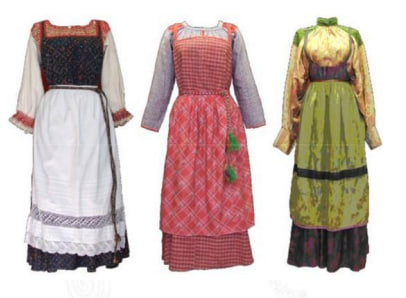
\includegraphics[width=0.5\textwidth]{images/f}
	\end{wrapfigure}
	
	Основа женского костюма – сочетание сарафана (сарапана) и рубахи. Поверх сарафана надевают запон (передник) и подпоясываются. Сарафан может быть разного кроя. Наиболее старинный – косоклинный.\\\\\\\\\\
	
	\pagebreak
	\begin{wrapfigure}{r}{0.5\textwidth}
		\centering
		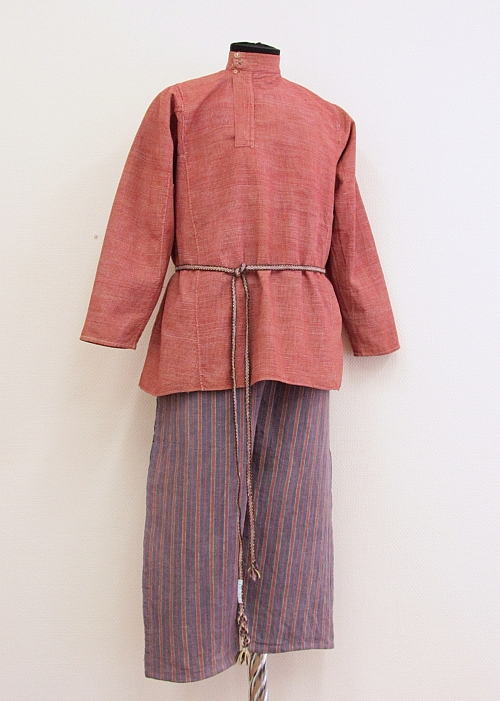
\includegraphics[width=0.25\textwidth]{images/m}
	\end{wrapfigure}
	
	Основа мужского костюма, как и женского, – рубаха. В старину рубахи были длиной до колен, туникообразного покроя. Носили их навыпуск, завязывая сверху пояс. По мере того, как мода менялась, рубахи становились короче, а в начале ХХ века вошли в моду косоворотки со стоячим воротником.\\
	
	\begin{wrapfigure}{l}{0.5\textwidth}
		\centering
		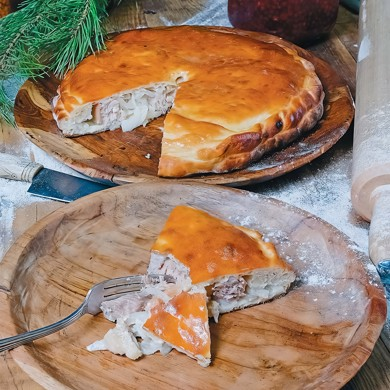
\includegraphics[width=0.3\textwidth]{images/ch}
	\end{wrapfigure}
	
	Одним из традиционных блюд коми является черинянь, но же рыбный пирог или рыбник. Главными ингредиентами являются тесто и рыба. Также традиционным блюдом является шаньга.\\\\\\
	
	Традиционное жилище коми представляло собой наземную, прямоугольную по форме, срубную из сосновых бревен постройку на высоком подклете (керка). Жилая часть состояла из зимней и летней изб, соединенных сенями. Характерная черта жилища -- односкатность крыши. В западных районах избы ставились так, что их односкатные крыши смыкались над домом в единую двускатную кровлю.
	
	\begin{figure}[h]
		\centering
		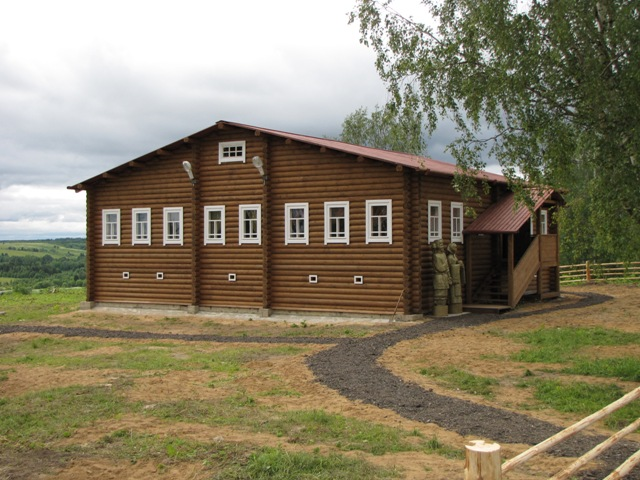
\includegraphics[width=0.5\textwidth]{images/h}
	\end{figure}
	
	\pagebreak
	Список литературы:
	
	\begin{enumerate}
		\item \href{https://ru.wikipedia.org/wiki/%D0%9A%D0%BE%D0%BC%D0%B8_(%D0%BD%D0%B0%D1%80%D0%BE%D0%B4)}{Коми (народ) - Материал из Википедии — свободной энциклопедии}
		
		\item \href{https://www.visitkomi.ru/region/tradicii_byt/}{Традиции и быт коми народа}
		
		\item \href{https://kraeveds.wixsite.com/mykrayrodnoy/komi-prazdniki}{Народные праздники Республики Коми}
		
		\item \href{https://arctic-children.com/article/pas-sarapan-i-toboki/}{Традиционный костюм народа коми}
		
		\item \href{https://eda.ru/recepty/vypechka-deserty/cherinyan-ili-tradicionnyy-rybnyy-pirog-komi-zyryan-125079}{Черинянь, или традиционный рыбный пирог коми-зырян}
	\end{enumerate}
\end{document}